\section{有效集法（Active-Set）}
\label{sec:sqp-active-set}

等式QP一步就能解完。不等式的困难在于事先不知道解处哪些不等式取等号：如果知道，把它们当等式，其余的扔掉，就回到了上一节。接下来要弄清：怎样一边迭代、一边找出这些约束？

这就像按预算线分配资源。有些预算在最优方案中被用尽，是真正起作用的边界；有些还有富余，暂时可以当它不存在。麻烦在于，只有解出方案后才知道哪些用尽了。有效集法的做法是先猜一组，解一下，看哪里不对，再改这一组。这个类比的边界是，算法改的是它自己维护的集合，这个集合不必与当前点真实触碰的边界完全相同。

\paragraph{要解的QP}
本节讨论一个独立的QP，记号与局部模型无关，变量写作$\bm{x}$：
\begin{equation}
 \min_{\bm{x}\in\mathbb{R}^n}\ q(\bm{x})=\frac12\bm{x}^\top\bm{B}\bm{x}+\langle\bm{c},\bm{x}\rangle
 \quad\text{s.t.}\quad\langle\bm{a}_i,\bm{x}\rangle\leq b_i,\quad i=1,\ldots,m.
 \label{eq:sqp-as-qp}
\end{equation}
等式约束若有，始终留在下面要定义的集合里，写法上不必单列。全节的例子是平面上到点$\bm{c}^\circ=(4,2)^\top$的投影：
\begin{equation}
 \begin{gathered}
 q(\bm{x})=\frac12\lVert\bm{x}-\bm{c}^\circ\rVert_2^2,\\
 g_1:\ x_1+x_2\leq3,\quad g_2:\ -x_1\leq0,\quad g_3:\ -x_2\leq0,\quad g_4:\ x_1+2x_2\leq4.
 \end{gathered}
 \label{eq:sqp-as-example}
\end{equation}
它的$\bm{B}=\bm{I}$，$\bm{c}=-\bm{c}^\circ$，可行域是顶点为$(0,0),(3,0),(2,1),(0,2)$的四边形。

\paragraph{活动约束与工作集}
先把两个容易混淆的集合分开。在可行点$\bm{x}$处，取等号的约束构成\term{活动集}（active set），它由$\bm{x}$决定。算法还维护一个下标集合$\bm{W}$，这一轮把其中的约束当等式处理，它称为\term{工作集}（working set），由算法的历史决定。

可行点上工作集总是活动集的子集，但两者不必相等。图~\ref{fig:sqp-active-vs-working}给出三种情形：(a)~点贴着$g_3$的边，$g_3$活动，算法却可能没把它放进工作集；(b)~在顶点$(3,0)$处两条约束都活动，工作集可以只含其中一条；(c)~两者重合。到了解处，算法想要的是工作集恰好为那些乘子为正的约束。

\begin{BookInlineFigure}
 \centering
 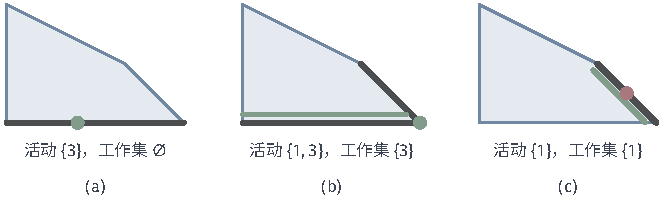
\includegraphics[width=112mm]{figures/05-optimization/06-constrained-optimization/tikz/sqp-active-vs-working/figure.pdf}
 \caption{活动集与工作集的区别，可行域取例~\eqref{eq:sqp-as-example}的四边形。深灰粗线是当前点真实触碰的边，绿色细带标出算法放进工作集的约束，圆点是当前点（红点为解）。}
 \label{fig:sqp-active-vs-working}
\end{BookInlineFigure}

\subsection{工作集的更新}
\label{sec:sqp-working-set}

本小节假设$\bm{B}\succ\bm{0}$，并且工作集中的约束梯度始终线性无关，已有一个可行的初始点。这样的初始点可以用第~\ref{chap:simplex-method}章两阶段法那样的辅助问题找到。

\paragraph{主要思想}
设$\bm{x}^{(t)}$可行，工作集为$\bm{W}$。把$\bm{W}$中的约束当等式，其余的先不管，问“从这里出发沿这张面能走到哪里”。写成对步$\bm{d}$的等式QP，并利用$\nabla q(\bm{x}^{(t)})=\bm{B}\bm{x}^{(t)}+\bm{c}$：
\begin{equation}
 \min_{\bm{d}}\ \frac12\bm{d}^\top\bm{B}\bm{d}+\langle\nabla q(\bm{x}^{(t)}),\bm{d}\rangle
 \quad\text{s.t.}\quad\langle\bm{a}_i,\bm{d}\rangle=0,\quad i\in\bm{W}.
 \label{eq:sqp-as-eqp}
\end{equation}
约束里右端是$0$，因为$\bm{W}$中的约束已经取等号，步不能破坏它们。结果分两种情况。

第一种，$\bm{d}\neq\bm{0}$。沿$\bm{d}$能降低$q$，但工作集以外的约束可能挡路。$\bm{W}$以外的约束$i$只在$\langle\bm{a}_i,\bm{d}\rangle>0$时才会变紧，走到边界所允许的比例是$(b_i-\langle\bm{a}_i,\bm{x}^{(t)}\rangle)/\langle\bm{a}_i,\bm{d}\rangle$。取其中最小的一个，并且不超过$1$，得到\term{比值检验}（ratio test）：
\begin{equation}
 \alpha^{(t)}=\min\Bigl\{1,\ \min_{i\notin\bm{W},\,\langle\bm{a}_i,\bm{d}\rangle>0}
 \frac{b_i-\langle\bm{a}_i,\bm{x}^{(t)}\rangle}{\langle\bm{a}_i,\bm{d}\rangle}\Bigr\}.
 \label{eq:sqp-ratio}
\end{equation}
新点是$\bm{x}^{(t)}$加上$\alpha^{(t)}\bm{d}$。若$\alpha^{(t)}<1$，取到最小值的约束称为\term{阻挡约束}（blocking constraint），把它加入工作集。它满足$\langle\bm{a}_b,\bm{d}\rangle>0$，而$\bm{W}$中的约束都有$\langle\bm{a}_i,\bm{d}\rangle=0$，所以它不在$\bm{W}$的约束梯度张成的子空间内，加入后仍线性无关。

第二种，$\bm{d}=\bm{0}$。当前点已是这张面上的最小点，该看乘子了。方程~\eqref{eq:sqp-kkt-system}的第一行此时给出
\begin{equation}
 \bm{B}\bm{x}^{(t)}+\bm{c}+\sum_{i\in\bm{W}}\lambda_i\bm{a}_i=\bm{0}.
 \label{eq:sqp-as-multiplier}
\end{equation}
若所有$\lambda_i\geq0$，再令$\bm{W}$以外的乘子为零，KKT条件全部成立，$\bm{B}\succ\bm{0}$时这就是全局最优解。

若有某个$\lambda_k<0$，负乘子说明这条约束不该被按住：它的影子价格是负的，相当于“放松这条预算，成本反而升高”，反过来说，向可行域内部离开这条边能让目标下降。下面的引理把这句话说准。

\begin{lemma}[释放负乘子约束]
\label{lem:sqp-drop}
设$\bm{d}=\bm{0}$时的乘子满足$\lambda_k<0$，令$\bm{W}'=\bm{W}\setminus\{k\}$，并设$\bm{d}'$是把$\bm{W}$换成$\bm{W}'$后问题~\eqref{eq:sqp-as-eqp}的解。则$\bm{d}'\neq\bm{0}$，$\bm{d}'$严格降低$q$的模型，并且
\begin{equation}
 \langle\bm{a}_k,\bm{d}'\rangle<0.
 \label{eq:sqp-drop-direction}
\end{equation}
\end{lemma}

\begin{proof}
先证$\bm{d}'\neq\bm{0}$。若$\bm{d}'=\bm{0}$，则存在系数$\mu_i$使$\nabla q+\sum_{i\in\bm{W}'}\mu_i\bm{a}_i=\bm{0}$。把它与式~\eqref{eq:sqp-as-multiplier}相减，得到$\bm{W}$中约束梯度的一个线性关系，其中$\bm{a}_k$的系数是$\lambda_k\neq0$，与线性无关矛盾。

再看方向。$\bm{d}'$的驻定条件是
\[
 \bm{B}\bm{d}'+\nabla q+\sum_{i\in\bm{W}'}\mu_i\bm{a}_i=\bm{0}.
\]

把式~\eqref{eq:sqp-as-multiplier}中的$\nabla q$代入，得
\[
 \bm{B}\bm{d}'=\sum_{i\in\bm{W}'}(\lambda_i-\mu_i)\bm{a}_i+\lambda_k\bm{a}_k.
\]

用$(\bm{d}')^\top$左乘，并注意$i\in\bm{W}'$时$\langle\bm{a}_i,\bm{d}'\rangle=0$，得到
\[
 (\bm{d}')^\top\bm{B}\bm{d}'=\lambda_k\langle\bm{a}_k,\bm{d}'\rangle.
\]
左端为正，$\lambda_k<0$，所以式~\eqref{eq:sqp-drop-direction}成立。

最后，$\bm{d}'$是等式QP的最小点而$\bm{d}=\bm{0}$可行，且最小点唯一，所以模型值严格小于零，即严格小于$\bm{d}=\bm{0}$时的模型值。
\end{proof}

式~\eqref{eq:sqp-drop-direction}的含义是，走$\bm{d}'$时被释放的约束$k$严格变松，点确实离开了这条边，不会立刻违反它。图~\ref{fig:sqp-activeset-multiplier}是例子中的这两个时刻。

\begin{BookInlineFigure}
 \centering
 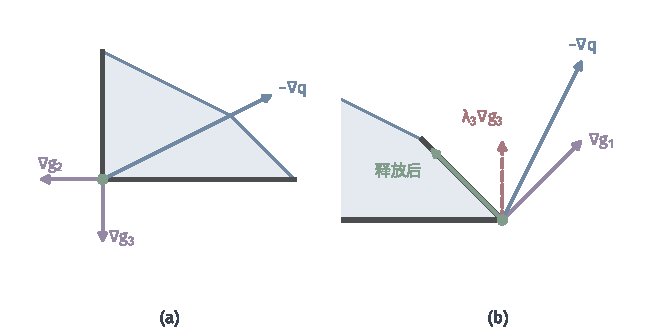
\includegraphics[width=112mm]{figures/05-optimization/06-constrained-optimization/matplotlib/sqp-activeset-multiplier/figure.pdf}
 \caption{乘子的符号。蓝色箭头是$-\nabla q$，紫色箭头是工作集约束的梯度，深灰粗线是工作集对应的边。(a)~原点处$-\nabla q=(4,2)^\top$指向可行域内部，它分解到两个向外的梯度上时系数都是负的。(b)~顶点$(3,0)^\top$处，$-\nabla q=\nabla g_1+\lambda_3\nabla g_3$，其中$\lambda_1=1$，$\lambda_3=-1$；红色虚线箭头是$\lambda_3\nabla g_3$。释放$g_3$后沿$g_1$的边（绿）走。}
 \label{fig:sqp-activeset-multiplier}
\end{BookInlineFigure}

整个逻辑可以画成图~\ref{fig:sqp-activeset-flow}。每一轮只改动工作集中的一条约束，或者加入一条，或者释放一条。

\begin{BookInlineFigure}
 \centering
 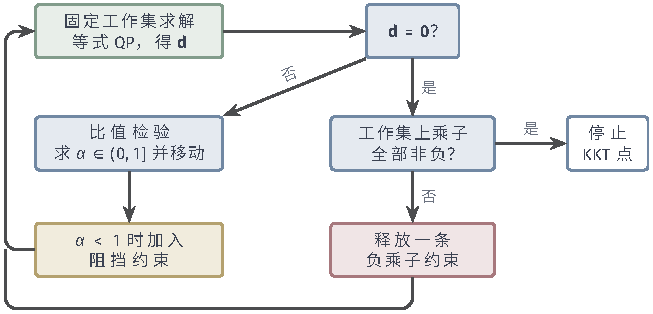
\includegraphics[width=112mm]{figures/05-optimization/06-constrained-optimization/tikz/sqp-activeset-flow/figure.pdf}
 \caption{有效集法一轮的判断。先求步；步非零则做比值检验，受阻时加入一条约束；步为零则看乘子，全部非负时停止，否则释放一条负乘子约束。}
 \label{fig:sqp-activeset-flow}
\end{BookInlineFigure}

\needspace{6\baselineskip}
\paragraph{变量}
\begin{itemize}
 \item $\bm{x}^{(t)}\in\mathbb{R}^n$：当前可行点。
 \item $\bm{W}$：工作集，下标集合，其大小不超过$n$。
 \item $\bm{A}_{\bm{W}}$：以$\bm{a}_i^\top$（$i\in\bm{W}$）为行的矩阵；$\bm{Z}_{\bm{W}}$：其零空间的基。
 \item $\bm{d}^{(t)}\in\mathbb{R}^n$：等式QP的解；$\lambda_i$（$i\in\bm{W}$）：工作集上的乘子。
\end{itemize}

\paragraph{初始化}
取可行点$\bm{x}^{(0)}$和一个工作集$\bm{W}$，其约束在$\bm{x}^{(0)}$处活动且梯度线性无关。例中取原点和它处的两条活动约束：
\[
 \bm{x}^{(0)}=(0,0)^\top,\qquad\bm{W}=\{2,3\}.
\]
目标值是$q(\bm{x}^{(0)})=10$。

\needspace{6\baselineskip}
\paragraph{每轮更新}
\begin{enumerate}
 \item 求步。由式~\eqref{eq:sqp-reduced-step}，取$\bm{h}=\bm{0}$，等式QP的解是
 \begin{equation}
  \bm{d}^{(t)}=-\bm{Z}_{\bm{W}}\bigl(\bm{Z}_{\bm{W}}^\top\bm{B}\bm{Z}_{\bm{W}}\bigr)^{-1}\bm{Z}_{\bm{W}}^\top\bigl(\bm{B}\bm{x}^{(t)}+\bm{c}\bigr).
  \label{eq:sqp-as-step}
 \end{equation}
 例中第一轮$\bm{W}=\{2,3\}$，零空间只有零向量，$\bm{d}^{(0)}=\bm{0}$。

 \item 若$\bm{d}^{(t)}=\bm{0}$，由式~\eqref{eq:sqp-as-multiplier}解出$\lambda_i$。行满秩时，用$\bm{A}_{\bm{W}}$左乘即得
 \begin{equation}
  \bm{\lambda}_{\bm{W}}=-\bigl(\bm{A}_{\bm{W}}\bm{A}_{\bm{W}}^\top\bigr)^{-1}\bm{A}_{\bm{W}}\bigl(\bm{B}\bm{x}^{(t)}+\bm{c}\bigr).
  \label{eq:sqp-as-lambda}
 \end{equation}
 全部非负就停止；否则从$\bm{W}$中去掉乘子最小的约束，令$\bm{x}^{(t+1)}=\bm{x}^{(t)}$，进入下一轮。

 例中第一轮$\nabla q=(-4,-2)^\top$，方程~\eqref{eq:sqp-as-multiplier}给出$\lambda_2=-4$，$\lambda_3=-2$。两个都是负的，释放$g_2$，得$\bm{W}=\{3\}$，$\bm{x}^{(1)}=\bm{x}^{(0)}$。

 \item 若$\bm{d}^{(t)}\neq\bm{0}$，由式~\eqref{eq:sqp-ratio}算$\alpha^{(t)}$，并移动到
 \begin{equation}
  \bm{x}^{(t+1)}=\bm{x}^{(t)}+\alpha^{(t)}\bm{d}^{(t)}.
  \label{eq:sqp-as-move}
 \end{equation}
 若$\alpha^{(t)}<1$，把阻挡约束加入$\bm{W}$。

 例中第二轮$\bm{W}=\{3\}$，$\bm{Z}_{\bm{W}}=(1,0)^\top$，由式~\eqref{eq:sqp-as-step}得$\bm{d}^{(1)}=(4,0)^\top$。比值检验只看$\langle\bm{a}_i,\bm{d}\rangle>0$的$g_1$和$g_4$：
 \[
  g_1:\ \frac{3}{4}=0.75,\qquad g_4:\ \frac{4}{4}=1.
 \]
 于是$\alpha^{(1)}=0.75$，受阻于$g_1$，得
 \[
  \bm{x}^{(2)}=(3,0)^\top,\qquad\bm{W}=\{1,3\},\qquad q(\bm{x}^{(2)})=2.5.
 \]

 第三轮零空间又只有零向量，$\bm{d}^{(2)}=\bm{0}$。此时$\nabla q=(-1,-2)^\top$，乘子满足
 \[
  \begin{bmatrix}-1\\-2\end{bmatrix}+\lambda_1\begin{bmatrix}1\\1\end{bmatrix}+\lambda_3\begin{bmatrix}0\\-1\end{bmatrix}=\bm{0}.
 \]
 第一行给$\lambda_1=1$，第二行给$\lambda_3=-1$。释放$g_3$，得$\bm{W}=\{1\}$，$\bm{x}^{(3)}=\bm{x}^{(2)}$。

 第四轮$\bm{Z}_{\bm{W}}=(1,-1)^\top$，$\bm{Z}_{\bm{W}}^\top\bm{Z}_{\bm{W}}=2$，$\bm{Z}_{\bm{W}}^\top\nabla q=1$。由式~\eqref{eq:sqp-as-step}，
 \[
  \bm{d}^{(3)}=-\frac12\begin{bmatrix}1\\-1\end{bmatrix}=(-0.5,\ 0.5)^\top.
 \]
 比值检验中$g_2$的比值是$3/0.5=6$，$g_4$的比值是$1/0.5=2$，都大于$1$，所以走满一步：
 \[
  \bm{x}^{(4)}=(2.5,\ 0.5)^\top,\qquad q(\bm{x}^{(4)})=2.25.
 \]

 \item 重复第1至3步，直到第2步发现乘子全部非负。

 例中第五轮$\bm{W}=\{1\}$，此时$\nabla q=(-1.5,-1.5)^\top$与$\bm{Z}_{\bm{W}}$正交，所以这一轮的步为零。乘子由下式确定：
 \[
  \nabla q+\lambda_1(1,1)^\top=\bm{0},\qquad\lambda_1=1.5\geq0.
 \]
 乘子非负，停止。
\end{enumerate}

最终得到$\bm{x}^\star=(2.5,0.5)^\top$，$g_1$是唯一的活动约束，影子价格$\lambda_1=1.5$。路径如图~\ref{fig:sqp-activeset-path}，每个停留的点上都发生一次工作集的变动。

\begin{BookInlineFigure}
 \centering
 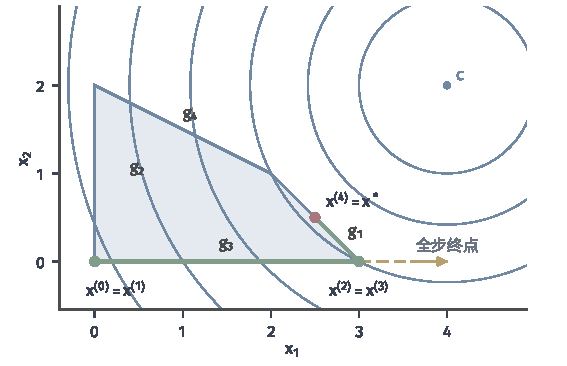
\includegraphics[width=96mm]{figures/05-optimization/06-constrained-optimization/matplotlib/sqp-activeset-path/figure.pdf}
 \caption{例~\eqref{eq:sqp-as-example}上有效集法的路径（绿）。浅蓝区域是可行域，蓝色同心圆是$q$的等高线，蓝点是无约束最小点$\bm{c}^\circ$。沿$g_3$的边本想走到$(4,0)^\top$（黄色虚线），在$(3,0)^\top$被$g_1$挡住；释放$g_3$后沿$g_1$走到红点，算法结束。}
 \label{fig:sqp-activeset-path}
\end{BookInlineFigure}

\paragraph{为什么有限步结束}
工作集的取法只有有限多种，只要同一个工作集不会被重复“解完”，算法就会停。

\begin{theorem}[有效集法的有限终止]
\label{thm:sqp-as-finite}
设$\bm{B}\succ\bm{0}$，工作集中的约束梯度始终线性无关，并且每个$\bm{d}^{(t)}\neq\bm{0}$的轮次都有$\alpha^{(t)}>0$。则算法在有限轮后停在问题~\eqref{eq:sqp-as-qp}的全局最优解。
\end{theorem}

\begin{proof}
称$\bm{d}^{(t)}=\bm{0}$的轮次为到站。两次到站之间，$\bm{W}$只增不减，所以至多有$n$轮比值检验，否则$\bm{W}$的大小超过$n$，与线性无关矛盾。由此到站必然反复发生或算法停止。

下面说明工作集不会在两次到站时重复。到站时$\bm{x}^{(t)}$是$q$在工作集约束所定义的仿射面上的唯一最小点，所以到站时的目标值由$\bm{W}$决定。

由引理~\ref{lem:sqp-drop}，到站后释放一条约束得到的步非零，严格降低模型。凸二次函数沿下降方向走$\alpha\in(0,1]$仍严格下降，而假设保证$\alpha>0$。所以相邻两次到站的目标值严格递减，同一个$\bm{W}$不会出现两次。工作集的个数有限，算法必在有限轮后到站且乘子全部非负，此时KKT条件成立，由凸性得全局最优。
\end{proof}

定理要求每次移动的步长为正。这个条件失效时会发生什么，是下面要讨论的。

\paragraph{退化、平局与热启动}
假设例中$g_4$改成$x_1+2x_2\leq3$。第二轮的比值检验中，$g_1$和$g_4$的比值都是$0.75$，出现平局，只能加入一条，另一条在下一点也活动却不在工作集中。

这一点已经是退化的：图~\ref{fig:sqp-degenerate}(b)那样，过一点的活动约束多于$n$条或梯度线性相关。这时比值检验可能算出$\alpha^{(t)}=0$，点不动，只有工作集换了一条。一连串这样的零步有可能转回原来的工作集，形成循环，定理的条件也就破坏了。

\begin{BookInlineFigure}
 \centering
 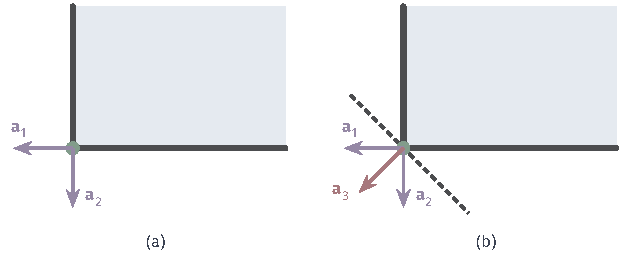
\includegraphics[width=100mm]{figures/05-optimization/06-constrained-optimization/tikz/sqp-degenerate/figure.pdf}
 \caption{顶点处的约束梯度。(a)~两条活动约束，紫色梯度线性无关，工作集的选取没有歧义。(b)~第三条约束（虚线）也经过同一点，三个梯度在平面内线性相关，工作集只能放下其中两条，走零步时点不动而工作集在变。}
 \label{fig:sqp-degenerate}
\end{BookInlineFigure}

实用的防范办法有两类。一类是确定性的选取规则，例如第~\ref{chap:simplex-method}章的Bland规则，在平局和释放时都按下标的固定顺序挑选，避免转圈。另一类是给约束右端加很小的扰动，让重合的边界分开，结束后再回到原数据上核对。释放时取最负的乘子是常用的选择，但它本身不防止循环。

有效集法还有一个明显的长处。如果手里有一个接近解的工作集，从它开始往往几轮就结束，这叫\term{热启动}（warm start）。SQP相邻两轮的QP数据只有微小变化，上一轮的工作集正是下一轮的好起点。内点法从内部出发，较难利用这种信息。每轮工作集只变一条约束，$\bm{K}$或$\bm{Z}$的分解也可以用低秩修正更新，不必重新分解。

\subsection{有效集法与SQP}
\label{sec:sqp-active-set-sqp}

把有效集法用在局部QP~\eqref{eq:sqp-qp}上时，变量是$\bm{d}$，$\bm{a}_i=\nabla g_i^{(t)}$，$b_i=-g_i^{(t)}$。本小节要回答的问题是：这样得到的工作集，和原问题解处真正活动的约束是什么关系？

\paragraph{工作集属于当前的线性化QP}
先看一个带不等式的例子，把问题~\eqref{eq:sqp-circle}的约束放宽，再加两条线性约束：
\begin{equation}
 \begin{gathered}
 \min_{\bm{x}}\ -x_1-x_2\\
 \text{s.t.}\quad g_1=x_1^2+x_2^2-2\leq0,\quad g_2=x_2-1.2\leq0,\quad g_3=-x_1\leq0.
 \end{gathered}
 \label{eq:sqp-ineq-example}
\end{equation}
解仍是$(1,1)^\top$，只有$g_1$活动，乘子$\lambda_1^\star=1/2$。下面用精确的Lagrange Hessian和全步长，从$\bm{x}^{(0)}=(0.5,1.7)^\top$、$\bm{\lambda}^{(0)}=(1,0,0)^\top$出发。

第一轮$\bm{B}^{(0)}=2\lambda_1^{(0)}\bm{I}=2\bm{I}$，约束的值和线性化约束是
\[
 \begin{gathered}
 g_1=1.14,\qquad g_2=0.5,\qquad g_3=-0.5,\\
 1.14+d_1+3.4\,d_2\leq0,\qquad 0.5+d_2\leq0,\qquad -0.5-d_1\leq0.
 \end{gathered}
\]

模型的目标是$-d_1-d_2+d_1^2+d_2^2$。先试工作集$\{2\}$：取$d_2=-0.5$，$d_1$的最优值是$0.5$。检验其余约束，线性化的$g_1$值是
\[
 1.14+0.5+3.4\times(-0.5)=-0.06\leq0,
\]
线性化的$g_3$值是$-1\leq0$，都满足。乘子由第二个驻定方程$-1+2d_2+\hat\lambda_2=0$得$\hat\lambda_2=2\geq0$。所以QP的解是
\[
 \bm{d}^{(0)}=(0.5,\ -0.5)^\top,\qquad\hat{\bm{\lambda}}=(0,\ 2,\ 0)^\top,\qquad\bm{x}^{(1)}=(1,\ 1.2)^\top.
\]

这一步说明了两件事。其一，这一轮的工作集是$\{2\}$，而原问题解处活动的是$\{1\}$：工作集属于这一轮的线性化QP，不是对原问题的最终判断。其二，$\bm{d}^{(0)}$满足全部线性化约束，新点却有
\[
 g_1(\bm{x}^{(1)})=1+1.44-2=0.44>0.
\]
QP可行不代表原问题可行，图~\ref{fig:sqp-qp-vs-nonlinear}(a)画的就是这个缺口：步落在线性化的半平面内，却冲出了圆。

\begin{BookInlineFigure}
 \centering
 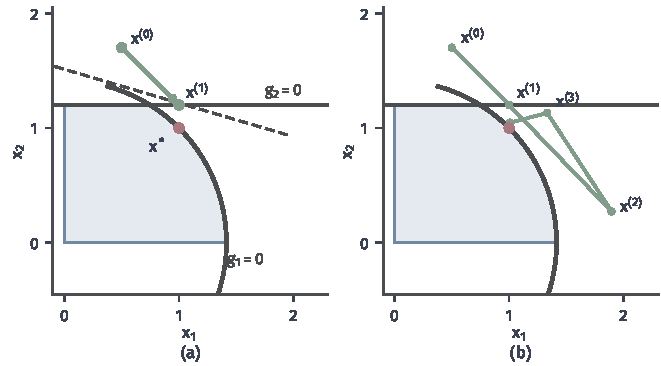
\includegraphics[width=112mm]{figures/05-optimization/06-constrained-optimization/matplotlib/sqp-qp-vs-nonlinear/figure.pdf}
 \caption{问题~\eqref{eq:sqp-ineq-example}上的SQP。浅蓝区域是真实可行域，深灰粗线是$g_1,g_2$的边界，绿色折线是迭代路径，红点是解。(a)~第一步，虚线是$g_1$在$\bm{x}^{(0)}$的线性化边界，$\bm{x}^{(1)}$满足线性化约束但在圆外。(b)~前五步的路径：工作集先后是$\{2\}$与$\{1\}$，迭代点在前几轮都不可行。}
 \label{fig:sqp-qp-vs-nonlinear}
\end{BookInlineFigure}

第二轮的乘子估计是$\lambda_1^{(1)}=0$，于是$\nabla^2_{\bm{x}\bm{x}}\mathcal{L}=\bm{0}$，子问题退化成线性规划。为了让子问题仍有曲率，这里临时取$\bm{B}^{(1)}=0.1\,\bm{I}$，这类修正下一节专门讨论。此后QP选中的工作集稳定为$\{1\}$，乘子很快接近$1/2$。图~\ref{fig:sqp-working-set-chart}列出各轮约束值和工作集。

\begin{BookInlineFigure}
 \centering
 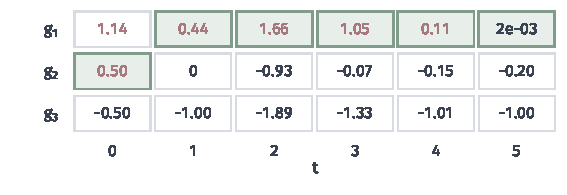
\includegraphics[width=96mm]{figures/05-optimization/06-constrained-optimization/matplotlib/sqp-working-set-chart/figure.pdf}
 \caption{问题~\eqref{eq:sqp-ineq-example}各轮的约束值$g_i(\bm{x}^{(t)})$，正值（红字）表示违反原约束，绿色格表示该约束在这一轮QP的最优工作集中。第一轮之后工作集稳定为$\{1\}$，而$g_1$的违反量要到后几轮才降下来。}
 \label{fig:sqp-working-set-chart}
\end{BookInlineFigure}

\paragraph{什么时候能认出解处的活动集}
图~\ref{fig:sqp-working-set-chart}的现象并不偶然。在解附近，QP的最优工作集会固定下来，且正好是原问题的活动集，此后的SQP就成了只含等式的SQP，上一节的结论都可以用。先复述第~\ref{chap:constrained-optimality}章的三个条件。设$(\bm{x}^\star,\bm{\lambda}^\star,\bm{\nu}^\star)$是KKT点，$\bm{S}^\star$是$\bm{x}^\star$处活动的不等式下标集。

\begin{itemize}
 \item 约束资格（LICQ）：活动不等式和全部等式的梯度在$\bm{x}^\star$处线性无关。
 \item 严格互补：对每个$i\in\bm{S}^\star$，有$\lambda_i^\star>0$。
 \item 二阶充分条件：$\nabla^2_{\bm{x}\bm{x}}\mathcal{L}$在解处沿活动约束梯度的零空间正定。在严格互补下，这就是该章临界锥上的二阶条件。
\end{itemize}

\begin{theorem}[解附近的活动集识别]
\label{thm:sqp-identification}
设上述三个条件成立。对任意有界的对称矩阵族$\{\bm{B}\}$，若它们在活动约束零空间上的约化矩阵一致正定，则存在$(\bm{x}^\star,\bm{\lambda}^\star,\bm{\nu}^\star)$的邻域，使得当当前点与乘子都在此邻域内时，QP~\eqref{eq:sqp-qp}有一个靠近$\bm{0}$的严格局部解$\bm{d}$，其活动集恰为$\bm{S}^\star$，乘子靠近$(\bm{\lambda}^\star,\bm{\nu}^\star)$。
\end{theorem}

\begin{proof}
把$\bm{S}^\star$中的不等式和全部等式都当作等式，写出方程~\eqref{eq:sqp-kkt-system}，其解记为$(\bm{d},\hat{\bm{\lambda}}_{\bm{S}^\star},\hat{\bm{\nu}})$，并令$\bm{S}^\star$以外的乘子为零。

由LICQ和约化矩阵的一致正定，KKT矩阵在该邻域内一致可逆（定理~\ref{thm:sqp-eqp}的论证与连续性）。在$(\bm{x}^\star,\bm{\lambda}^\star,\bm{\nu}^\star)$处方程右端使解为$\bm{d}=\bm{0}$，乘子为$(\bm{\lambda}^\star_{\bm{S}^\star},\bm{\nu}^\star)$。方程右端连续，而$\bm{B}\bm{d}$随$\bm{d}\to\bm{0}$趋于零，所以邻域足够小时$\bm{d}$靠近$\bm{0}$，乘子靠近其真值。

现在逐条核对条件~\eqref{eq:sqp-qp-kkt}。严格互补使$\hat\lambda_i>0$（$i\in\bm{S}^\star$），乘子符号成立。对$i\notin\bm{S}^\star$，有$g_i(\bm{x}^\star)<0$，由连续性$g_i+\langle\nabla g_i,\bm{d}\rangle<0$，这些约束严格满足。所以$\bm{d}$是QP的KKT点，活动集恰为$\bm{S}^\star$。

最后，活动约束的乘子严格为正，且$\bm{B}$在其零空间上正定，所以二阶充分条件对这个QP成立，$\bm{d}$是严格局部解。
\end{proof}

这个定理只断言“存在这样一个解”。QP非凸时可能还有别的局部解，求解器未必返回这一个；若从上一轮的工作集热启动，实际中通常就落在这一个上。条件各有其用：缺少严格互补时，$\lambda_i^\star=0$的约束可能在相邻两轮时进时出；缺少约束资格时乘子不唯一，方程组可能接近奇异。

\paragraph{原问题的检查不能省}
工作集稳定是解附近的现象，远离解时它可能频繁变动。即使稳定了，QP可行也只是切平面上的可行。所以有效集法解完子问题后，仍然要回到原问题检验新点的目标和约束，这正是第~\ref{sec:sqp-acceptance}节的内容。
